\beginsong{Straßen auf und Straßen ab}[
    wuw={George Forestier, helm (Helmut König)}, 
    pfii={17}, 
    pfiii={7}, 
    bo={300}, 
    gruen={62}, 
    kssiv={5}, 
    siru={224},
]

\beginverse
\endverse 
\centering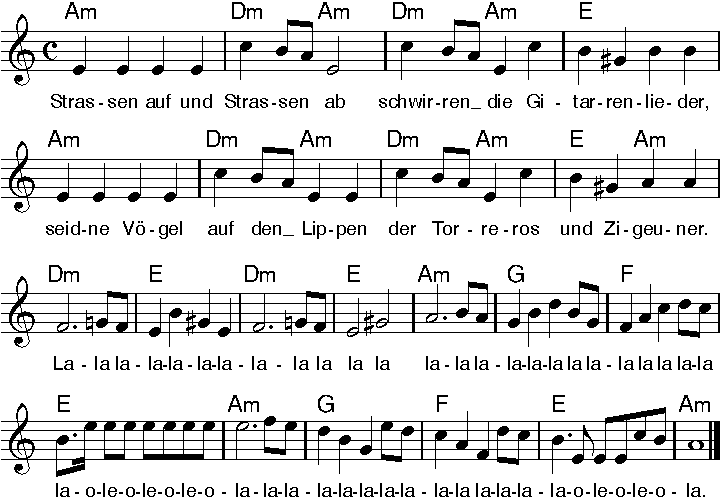
\includegraphics[width=1\textwidth]{Noten/Lied082.pdf}


\beginverse*
{\nolyrics Zwischenspiel: \[Am] \[G] \[F] \[E] } 
\endverse 

\beginverse\memorize
\[Am]Ebro auf und \[Dm]Ebro \[Am]ab, \[Dm]in der \[Am]Stunde \[E]der Orangen,
\[Am]lockt die Sonne \[Dm]Kata\[Am]loniens \[Dm]mit den \[Am]Rhythmen \[E]der Gi\[Am]tarren.
\endverse

\beginchorus
\[Dm]La lala \[E]lala \[Dm]la lala \[E]lala \[Am]la lala \[G]la lala \[F]la lala \[E]la o-le o-
le o-le o \[Am]la lala \[G]la lala \[F]la lala \[E]la o-le o-le o-\[Am]la.
{\nolyrics Zwischenspiel: \[Am] \[G] \[F] \[E] }
\endchorus

\beginverse
^In den Höfen ^der Pa^läste ^bröckelt ^von ver^gilbten Mauern,
schweigen die Gitarrenlieder klingen nicht in Saragossa.
\endverse

\printchorus

\beginverse
^Straßen auf und ^Straßen ^ab ^schwirren die ^Blicke ^der Verliebten,
^schwirren die Gi^tarren^lieder ^in der ^Stunde ^der O^rangen.
\endverse

\printchorus

\endsong

\beginscripture{}
Ebro = Fluss im Nordosten Spaniens; Katalonien = Region im Nordosten Spaniens; Saragossa = Stadt in Spanien entlang des Ebro
\endscripture
